% !TEX program = xelatex
\documentclass[12pt]{article}
\usepackage[a4paper, margin=2.45cm]{geometry}
\usepackage[fleqn]{amsmath}
\usepackage{amssymb}
\usepackage{amsfonts}
\usepackage[dvipsnames]{xcolor}
\usepackage{setspace}
\usepackage{graphicx}
\usepackage{cancel}
\usepackage{xfrac}
\usepackage{fontenc}
\usepackage{fontspec}
\usepackage[none]{hyphenat}
\usepackage{etoolbox}
\usepackage{longtable}
\usepackage{listings}
\usepackage{hyperref}

\hypersetup{
    colorlinks=true,
    linkcolor=blue,
    filecolor=magenta,      
    urlcolor=cyan,
}

\setlength{\LTleft}{0pt}
\lstset{basicstyle = \footnotesize\color{white}\ttfamily, backgroundcolor = \color{bg}}%, moredelim=**[is][\color{green}]{@}{@}, moredelim=**[is][\color{gray}]{*}{*}, moredelim=**[is][\color{black}]{/*}{/*}}
\AtBeginEnvironment{align}{\setcounter{equation}{0}}
\setmonofont{Consolas}
\everymath{\displaystyle}
\begin{document}
% \onehalfspacing
\definecolor{bg}{gray}{0.1}
% \pagecolor{bg}
% \color{white}
\newcommand{\unt}{\int\displaylimits}
\newcommand{\jadi}{$\therefore\;$}
\newcommand{\rut}[1]{\sqrt{#1}}
\newcommand{\jgj}{\Leftrightarrow}
\newcommand{\tebal}[1]{\underline{\textbf{#1}}\bigskip}
\newcommand{\infak}{\int\displaylimits^{\infty}_{\infty}}
\newcommand{\lqm}{\lim\displaylimits}

\sloppy

\noindent
2102800 - Muhammad Rahman Wicaksono - Pertemuan 2 Analisis Numerik\\
\noindent\rule{\textwidth}{0.2pt}\bigbreak

Diberikan persamaan sebagai berikut:
\begin{align*}
    x^2 = 3 + \ln(x)
\end{align*}
\begin{enumerate}
    \item {
        Bagaimana metode Newton-Raphson mencari hampiran akar-akar persamaan tak linier tersebut?\bigskip

        Untuk menggunakan metode Newton-Raphson, persamaan harus diubah menjadi bentuk fungsi $ f(x) = $ dan mencari solusinya. Lalu metode Newton-Raphson terhadap suatu fungsi $ f(x) $ dimulai dengan menetukan titik perkiraan awal $ x_0 $. Penentuan titik ini dapat dilakukan dengan metode grafik tunggal, metode grafik ganda, metode tabulasi, atau metode lainnya. Kemudian hitung hampiran solusi yang lebih baik yaitu
        \begin{align*}
            x_n = x_{n-1}\frac{f(x_n-1)}{f'(x_n-1)}
        \end{align*}
        Hal ini dilakukan berulang kali hingga kondisi berhenti yang diinginkan terpenuhi.\bigskip

        Untuk kasus $ x^2 = 3 + \ln(x) $, persamaan diubah menjadi fungsi $ f(x) $ yaitu
        \begin{align*}
            f(x) = 3 + \ln(x) - x^2
        \end{align*}
        Lalu untuk menetukan $ x_0 $, digunakan metode grafik tunggal
        \begin{center}
        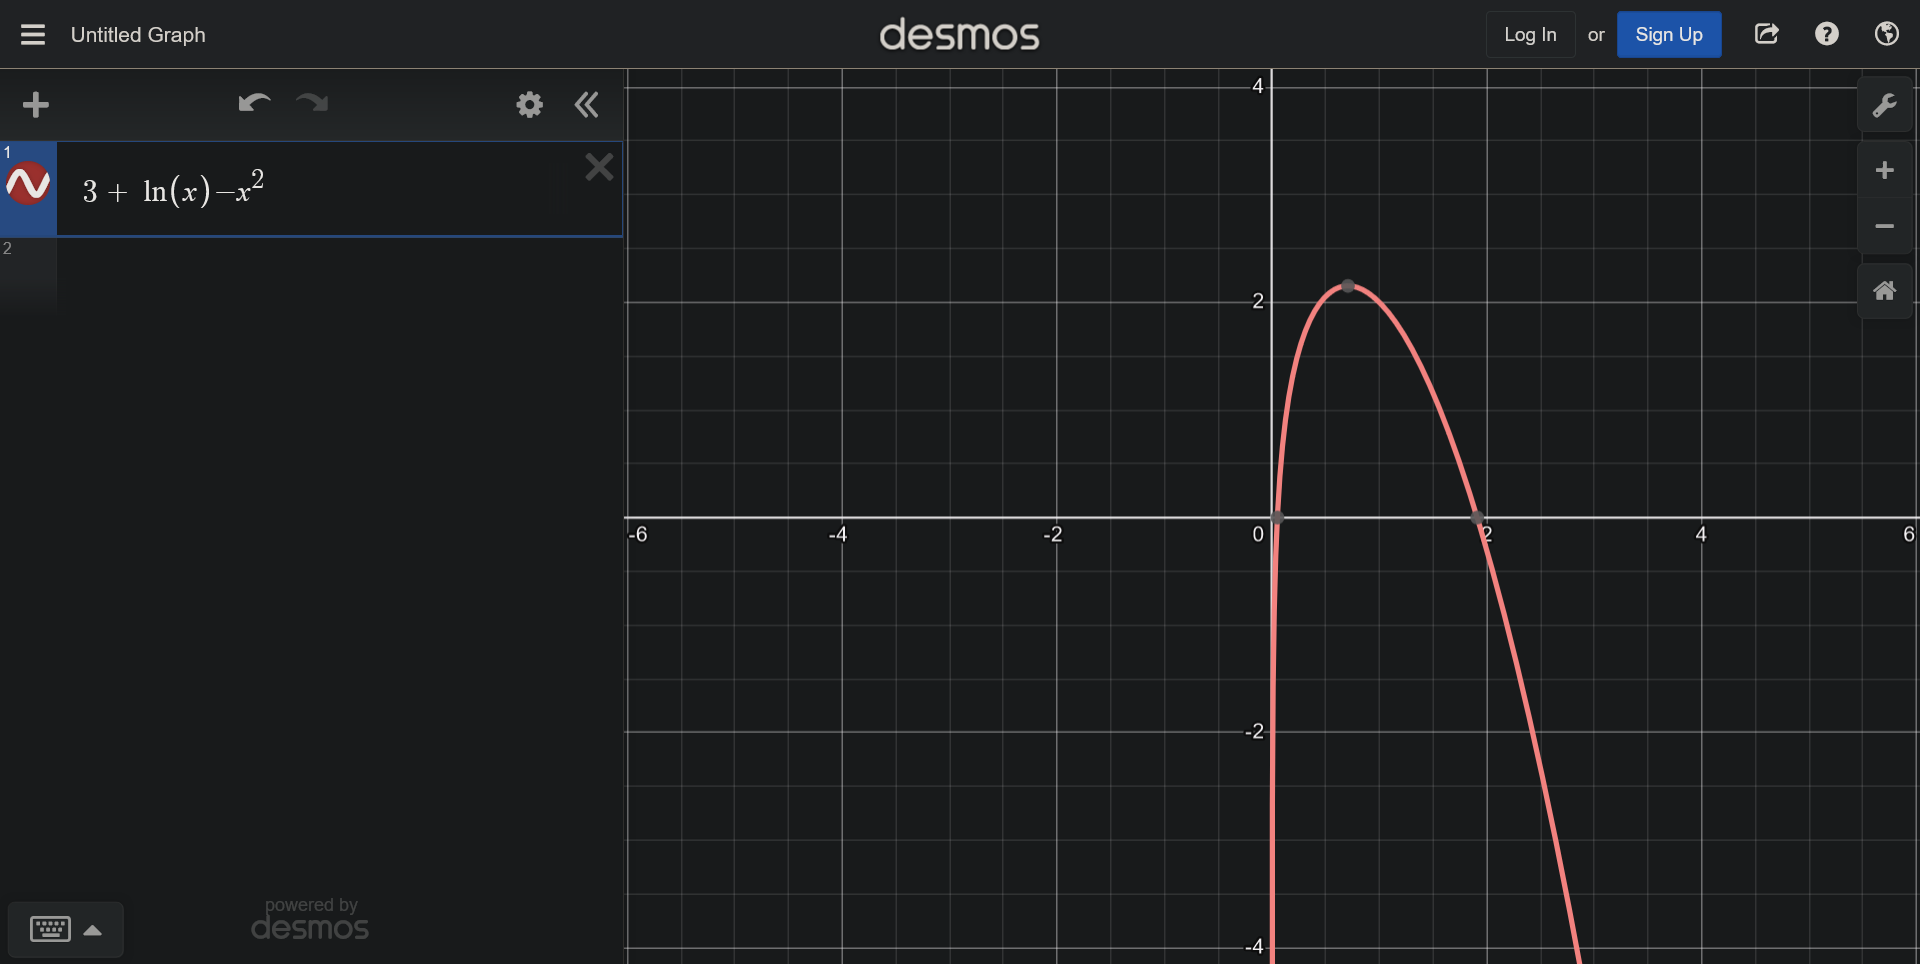
\includegraphics[scale = 0.2]{Screenshot 2023-09-13 at 23-13-48 Desmos Graphing Calculator.png}
        \end{center}
        Dari grafik diatas, terlihat bahwa $ f(x) $ memiliki akar solusi di sekitar 2. maka akan digunakan $ x_0 = 2 $. Untuk menghitung hampiran akar solusinya, digunakan bahasa pemograman "Rust" sebagai berikut
        \begin{lstlisting}
    use std::io;

    // INPUT KE VARIABEL
    fn read() -> String {
        let mut buffer = String::new();
        io::stdin().read_line(&mut buffer).expect("Failed");
        return buffer;
    }
    
    // FUNGSI F(X)
    fn f(x : f64) -> f64 {
        return 3.0 + x.ln() - (x * x);
    }
    
    // FUNGSI F'(X)
    fn f_(x : f64) -> f64 {
        return (1.0/x) - (2.0 * x)
    }
    
    fn main() {
    
        // INPUT X0
        println!("x0 =");
        let mut x : f64 = read()
            .trim()
            .parse()
            .expect("Not a real number!");
        while f_(x) == 0.0 {
            println!();
            println!("Invalid value");
            println!("x0 =");
            x = read()
                .trim()
                .parse()
                .expect("Not a real number!");
        }
    
        // INPUT GALAT
        println!();
        println!("Galat Mutlak =");
        let galat : f64 = read()
            .trim()
            .parse()
            .expect("Not a real number!");
    
        // INPUT GALAT RELATIF
        println!();
        println!("Galat Relatif");
        let galat_ : f64 = read()
            .trim()
            .parse()
            .expect("Not a real number!");
        
        // lOOPING ALGORITMA
        let mut iter = 0;
        while   (f(x) != 0.0) & 
                ((f(x)/f_(x)).abs() > galat) & 
                ((f(x)/(f_(x)*(x - (f(x)/f_(x))))).abs() > galat_) {
    
            {   // OUTPUT ITERASI
                println!();
                println!();
                println!("Iteras {iter}");
                println!();
                println!("x0       = {x}");
                println!("f(x0)    = {}", f(x));
                println!();
                println!("x        = {}", x - (f(x)/f_(x)));
                println!("|x - x0| = {}", (f(x)/f_(x)).abs());
            }
    
            // PERHITUNGAN ITERASI
            x = x - (f(x)/f_(x));
            iter = iter + 1;
        }
    
        {   // OUTPUT HASIL
            println!();
            println!();
            println!("Iteras {iter}");
            println!();
            println!("x0       = {x}");
            println!("f(x0)    = {}", f(x));
            println!();
            println!("x        = {}", x - (f(x)/f_(x)));
            println!("|x - x0| = {}", (f(x)/f_(x)).abs());
            println!();
            println!();
            println!("Solusi x = {x}");
        }
    }            
        \end{lstlisting}
        Perhitungan hampiran akar solusi dilakukan dengan galat mutlak dan galat relatif 0.0000001. Berikut hasil perhitungan tersebut
        \begin{lstlisting}
    x0 =
    2
    
    Galat Mutlak =
    0.0000001
    
    Galat Relatif
    0.0000001
    
    
    Iteras 0
    
    x0       = 2
    f(x0)    = -0.3068528194400546
    
    x        = 1.9123277658742701
    |x - x0| = 0.08767223412572989
    
    
    Iteras 1
    
    x0       = 1.9123277658742701
    f(x0)    = -0.008676258529709102
    
    x        = 1.9096999763093983
    |x - x0| = 0.0026277895648718287
    
    
    Iteras 2
    
    x0       = 1.9096999763093983
    f(x0)    = -0.000007850262289998966
    
    x        = 1.9096975943798067
    |x - x0| = 0.000002381929591525447
    
    
    Iteras 3
    
    x0       = 1.9096975943798067
    f(x0)    = -0.00000000000645128395149186
    
    x        = 1.9096975943778491
    |x - x0| = 0.0000000000019574542654168266
    
    
    Solusi x = 1.9096975943798067
        \end{lstlisting}
        Dari hasil diatas, diperoleh hampiran akar solusinya adalah $ x = 1.9096975943798067 $
    } \bigskip
    \item {
        Bagaimana metode Secant mencari hampiran akar-akar persamaan tak linier tersebut?\bigskip

        Untuk menggunakan metode Secant, persamaan harus diubah menjadi bentuk fungsi $ f(x) = $ dan mencari solusinya. Lalu metode Secant terhadap suatu fungsi $ f(x) $ dimulai dengan menetukan titik perkiraan awal $ x_0 $ dan $ x_1 $. Penentuan titik ini dapat dilakukan dengan metode grafik tunggal, metode grafik ganda, metode tabulasi, atau metode lainnya. Kemudian hitung hampiran solusi yang lebih baik yaitu
        \begin{align*}
            x_n = x_{n-1} - \frac{f(x_{n-1})(x_{n-1} - x_{n-2})}{f(x_{n-1}) - f(x_{n-2})}
        \end{align*}
        Hal ini dilakukan berulang kali hingga kondisi berhenti yang diinginkan terpenuhi.\bigskip

        Untuk kasus $ x^2 = 3 + \ln(x) $, persamaan diubah menjadi fungsi $ f(x) $ yaitu
        \begin{align*}
            f(x) = 3 + \ln(x) - x^2
        \end{align*}
        Lalu untuk menetukan $ x_0 $ dan $ x_1 $, digunakan metode grafik tunggal
        \begin{center}
        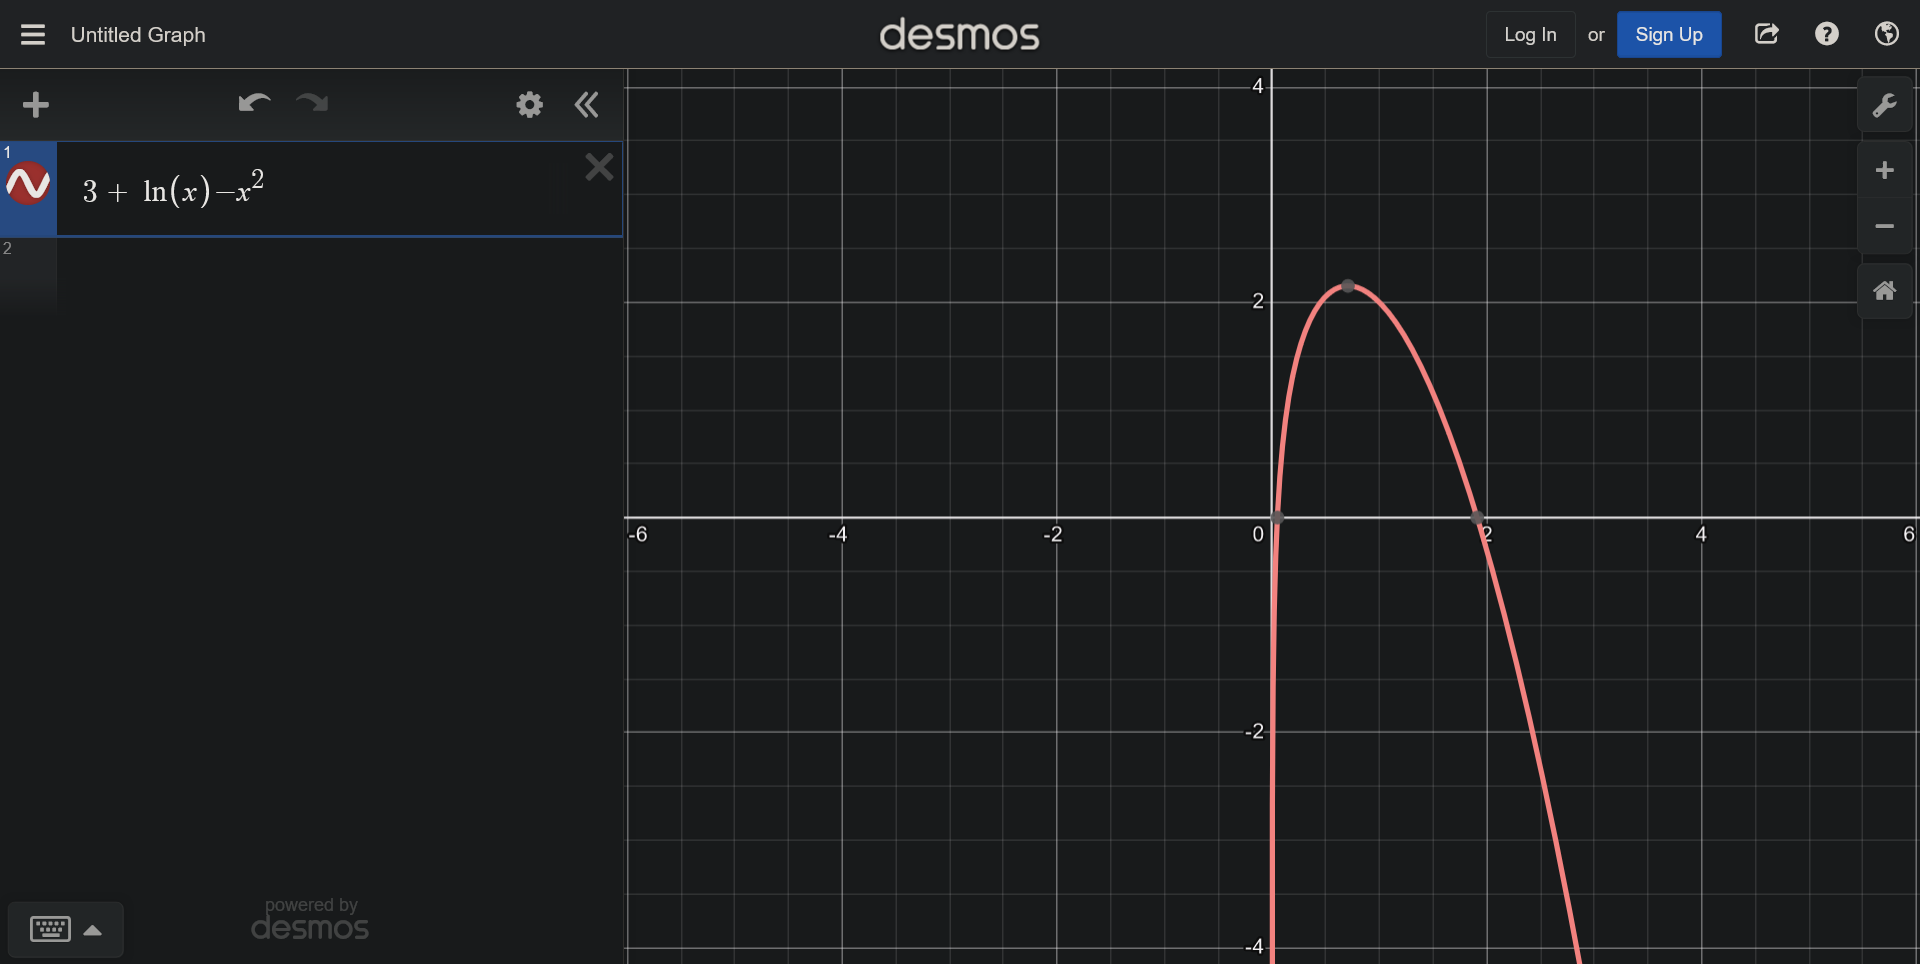
\includegraphics[scale = 0.2]{Screenshot 2023-09-13 at 23-13-48 Desmos Graphing Calculator.png}
        \end{center}
        Dari grafik diatas, terlihat bahwa $ f(x) $ memiliki akar solusi di sekitar 2. maka akan digunakan $ x_0 = 2 $ dan $ x_1 = 1.9 $. Untuk menghitung hampiran akar solusinya, digunakan bahasa pemograman "Rust" sebagai berikut
        \begin{lstlisting}
    use std::io;

    // INPUT KE VARIABEL
    fn read() -> String {
        let mut buffer = String::new();
        io::stdin().read_line(&mut buffer).expect("Failed");
        return buffer;
    }
    
    // FUNGSI F(X)
    fn f(x : f64) -> f64 {
        return 3.0 + x.ln() - (x * x);
    }
    
    fn main() {
    
        // INPUT X0
        println!();
        println!("x0 =");
        let mut x0 : f64 = read()
            .trim()
            .parse()
            .expect("Not a real number!");
    
        // INPUT X1
        println!();
        println!("x1 =");
        let mut x : f64 = read()
            .trim()
            .parse()
            .expect("Not a real number!");
    
        // VALIDASI X0 X1
        while f(x) == f(x0) {
            println!();
            println!();
            println!("Invalid");
            println!();
            println!("x0 =");
            x0 = read()
                .trim()
                .parse()
                .expect("Not a real number!");
            println!();
            println!("x1 =");
            x = read()
                .trim()
                .parse()
                .expect("Not a real number!");
        }
    
        // INPUT GALAT
        println!();
        println!("Galat Mutlak =");
        let galat : f64 = read()
            .trim()
            .parse()
            .expect("Not a real number!");
    
        // INPUT GALAT RELATIF
        println!();
        println!("Galat Relatif =");
        let galat_ : f64 = read()
            .trim()
            .parse()
            .expect("Not a real number!");
    
        // LOOPING ALGORITMA
        let mut iter = 0;
        while   (f(x) != 0.0) & 
                (f(x) != f(x0)) & 
                ((x - x0).abs() > galat) & 
                (((x - x0) / x).abs() > galat_) {
            
            {   // OUTPUT ITERASI
                println!();
                println!();
                println!("Iterasi {iter}");
                println!();
                println!("x{iter} = {x0}");
                println!("x{} = {x}",iter + 1);
                println!();
                println!("f(x{}) = {}", iter + 1, f(x));
                println!();
                println!("|x{} - x{iter}| = {}",iter+1,(x - x0).abs());
            }
    
            let buffer = x;
            x = x - (f(x) * (x - x0)) / (f(x) - f(x0));
            x0 = buffer;
            iter = iter + 1
        }
        {   // OUTPUT ITERASI
            println!();
            println!();
            println!("Iterasi {iter}");
            println!();
            println!("x{iter} = {x0}");
            println!("x{} = {x}",iter + 1);
            println!();
            println!("f(x{iter}) = {}", f(x));
            println!();
            println!("|x{} - x{iter}| = {}",iter+1,(x - x0).abs());
            println!();
            println!();
            println!("Solusi x = {x}");
            println!();
        }
    }            
        \end{lstlisting}
        Perhitungan hampiran akar solusi dilakukan dengan galat mutlak dan galat relatif 0.0000001. Berikut hasil perhitungan tersebut
        \begin{lstlisting}
    x0 =
    2
    
    x1 =
    1.9
    
    Galat Mutlak =
    0.0000001
    
    Galat Relatif =
    0.0000001
    
    
    Iterasi 0
    
    x0 = 2
    x1 = 1.9
    
    f(x1) = 0.03185388617239493
    
    |x1 - x0| = 0.10000000000000009
    
    
    Iterasi 1
    
    x1 = 1.9
    x2 = 1.9094045631942234
    
    f(x2) = 0.0009656604896810528
    
    |x2 - x1| = 0.009404563194223448
    
    
    Iterasi 2
    
    x2 = 1.9094045631942234
    x3 = 1.9096985786288636
    
    f(x3) = -0.000003243848421874418
    
    |x3 - x2| = 0.00029401543464024904
    
    
    Iterasi 3
    
    x3 = 1.9096985786288636
    x4 = 1.9096975942783285
    
    f(x4) = 0.0000000003279958527002691
    
    |x4 - x3| = 0.000000984350535082612
    
    
    Iterasi 4
    
    x4 = 1.9096975942783285
    x5 = 1.9096975943778494
    
    f(x4) = -0.0000000000000004440892098500626
    
    |x5 - x4| = 0.00000000009952083601660888
    
    
    Solusi x = 1.9096975943778494
        \end{lstlisting}
        Dari hasil diatas, diperoleh hampiran akar solusinya adalah $ x = 1.9096975943778494 $
    } \bigskip
    \item {
        Apa yang dapat kalian simpulkan mengenai metode-metode yang telah digunakan (metode bagi-dua, posisi palsu, Newton-Raphson, dan metode Secant) pada masalah penentuan hampiran akar untuk masalah tersebut? \bigskip

        Keempat metode tersebut memiliki kelebihan dan kekurangannya masing-masing yaitu
        \begin{enumerate}
            \item {
                Bagi-Dua \bigskip

                Metode ini mudah untuk dihitung namun membutuhkan iterasi lebih kecuali untuk kasus-kasus tertentu \bigskip
            }
            \item {
                Posisi Palsu \bigskip

                Metode ini lebih sulit untuk dihitung namun membutuhkan lebih sedikit iterasi. Selain itu metode ini berpotensi tidak menghasilkan apapun jika didapat titik mandek. \bigskip
            }
            \item {
                Newton-Raphson \bigskip

                Metode ini lebih sulit lagi dari kedua metode diatas, namun perhitungan tidak membutuhkan interval dan membutuhkan jumlah iterasi lebih sedikit. Kelemahan dari metode ini adalah berpotensi tidak menghasilkan apapun jika perhitungan yang dilakukan divergen \bigskip
            }
            \item {
                Secant \bigskip

                Sama seperti metode sebelumnya, metode ini tidak membutuhkan interval namun tetap membutuhkan 2 titk perkiraan awal. Sisi baiknya, potensi metode ini mengalami divergen lebih kecil dengan perbedaan jumlah iterasi dengan metode Newton-Raphson relatif kecil \bigskip
            }
        \end{enumerate}
    }
\end{enumerate}
Sumber : 
\begin{enumerate}
    \item Rinaldi Munir - Metode Numerik
    \item \href{https://en.wikipedia.org/wiki/Newton's_method}{Newton's method - Wikipedia}
    \item \href{https://en.wikipedia.org/wiki/Secant_method}{Secant method - Wikipedia}
\end{enumerate}
\end{document}